\begin{center}
    % First Assembly and CFG
    \begin{minipage}{0.22\textwidth}
    \begin{lstlisting}[style=AsmStyle]
triangleBranch:
  LDR R0, =x_
  LDR R1, [R0]
  ADD R1, R1, #1
  STR R1, [R0]
  CMP R1, #0
  BEQ FBB
  LDR R0, =x_
  MOV R1, #42
  STR R1, [R0]
FBB:
  LDR R0, =y_
  MOV R1, #100
  STR R1, [R0]
  BX LR
    \end{lstlisting}
    \end{minipage}
    \hfill
    \begin{minipage}{0.22\textwidth}
    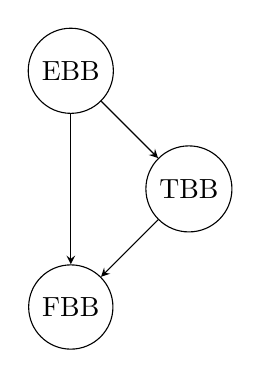
\begin{tikzpicture}[node distance=1.5cm and 2cm, >=stealth]
        \node[circle, draw, fill=white, minimum size=0.8cm] (EBB) at (0, 3) {EBB};
        \node[circle, draw, fill=white, minimum size=0.8cm] (TBB) at (1.5, 1.5) {TBB};
        \node[circle, draw, fill=white, minimum size=0.8cm] (FBB) at (0, 0) {FBB};

        \draw[->] (EBB) -- (TBB);
        \draw[->] (EBB) -- (FBB);
        \draw[->] (TBB) -- (FBB);
    \end{tikzpicture}
    \end{minipage}
    \hfill
    % Second Assembly and CFG
    \begin{minipage}{0.22\textwidth}
    \begin{lstlisting}[style=AsmStyle]
triangleBranch:
  LDR R0, =x_
  LDR R1, [R0]
  ADD R1, R1, #1
  STR R1, [R0]
  CMP R1, #0
  @@MOV R3, #42
  @MOV R4, #100
  @@IT NE
  @@MOVNE R1, R3
  @@MOVEQ R1, R4
  STR R1, [R0]
  LDR R0, =y_
  STR R4, [R0]
  BX LR
    \end{lstlisting}
    \end{minipage}
    \hfill
    \begin{minipage}{0.22\textwidth}
    
\begin{tikzpicture}[node distance=1.5cm and 2cm, >=stealth]
        \node[circle, draw, fill=white, minimum size=0.8cm] (EBB) at (0, 3) {EBB};
    \end{tikzpicture}
    \end{minipage}
    \end{center}